\subsection{JTL}
\label{sec:JTL}

\NOTE{\emph{Solution expert:} Romina, \emph{Interviewer:} Tony}


JTL (Janus Transformation Language)~\cite{CDEP10} is a constraint-based model transformation language specifically tailored to support bidirectionality and non-determinism. The implementation relies on the Answer Set Programming (ASP)~\cite{GL88}, which is a form of declarative programming oriented towards difficult (primarily NP-hard) search problems and based on the stable model (answer set) semantics of logic programming. 
JTL adopts a QVT-R~\cite{QVT-1.3} like syntax and allows a declarative specification of relationships between MOF models. The mechanism of transformation is rule-based; the language supports object pattern matching, and automatically generates trace links instances (i.e., traceability models) to record what occurred during a transformation execution~\cite{EPT18}. %A transformation between candidate models is specified as a set of \emph{relation}s that must hold for the transformation to be successful: in particular, it is defined by two \emph{domain}s and includes a pair of \emph{when} and \emph{where} predicates that specify the pre- and post- conditions that must be satisfied by the elements of the candidate models.  
%A transformation can be invoked for \emph{enforce}ment or as \emph{checkonly}. When invoked for enforcement, it is executed in a particular direction by selecting one of the candidate models as the target. A transformation can also be invoked in bidirectional mode by marking as enforcement both domain directions. 

The semantics is given in terms of ASP: an ASP transformation consists of a set of rules, which describe correspondences among element types of the source and target metamodels, and a set of constraints, which specify restrictions on the given correspondences.  Whereas, the transformation engine, also written in the ASP, is able to interpret the correspondences among elements and execute the transformation. Then, the ASP solver finds and generates, by a deductive process and in a single execution, all the possible models which are consistent with the transformation rules. 
 

The JTL framework~\cite{EPT18}
%~\footnote{JTL Tool: https://jtl.di.univaq.it} 
has been implemented within the Eclipse framework and mainly exploits Eclipse EMF. Moreover, it makes use of the DLV
%~\footnote{DLV-complex: https://www.mat.unical.it/dlv-complex/} 
solver~\cite{DLV} (which has been wrapped and integrated in the overall environment) to execute transformations in both forward and backward directions.


\subsubsection{Classification}
A summary of the features of JTL is provided in table~\ref{tab:features-all-tools}. Its architecture is \emph{restoration-based}.
%
The consistency can be restored both in forward and target directions by running the bidirectional transformation from the source or target model, respectively. Optionally, a traceability model (that collect the  states of the source and the target model in respect to a transformation execution) can be provided as input of the transformation execution. 
%
With respect to horizontal and vertical inputs, JTL realizes a \emph{state-state-based} architecture.

JTL requires to specify a consistency relation in \emph{explicit} way by defining bidirectional relations/rules and constraints. The same consistency relations are then used to perform a \emph{controlled} synchronization. It is a non-deterministic approach in which programmers need only to specify the consistency relation, allowing the engine to resolve the specification non-deterministically~\cite{monads}. This corresponds to generating all valid choices and letting the designer to identify the right one. In this respect, the bx notation has been generalized by adopting multivalued functions~\cite{EPR15} to capture the multiplicity of the solution space. In~\cite{EPR15}, also the definition of correctness and hippocraticness have been postulates according to the multiplicity of the solution space. In particular, JTL guarantees
\emph{correctness}: all the generated target solutions are consistent to the source model. Also, it guarantees \emph{hippocraticness}: the transformation not modify models if they are already in the specified consistency relation. 

JTL performs a \emph{directed} synchronization in both forward or backward direction and the approach is not incremental so that the direct synchronization creases the updated model from \emph{scratch}. Moreover, the synchronization is run in \emph{automatic} way without any user interaction and it is performed \emph{on-demand}.  



\subsubsection{Benchmark solution with JTL (draft)}


The Families-to-Persons bidirectional transformation written in JTL is reported in
Listing~\ref{lst:jtl}. The transformation is defined by means of relations defined among
elements of the two involved domains. In particular, on Line~\ref{lst:transf}, variables \code{family} and
\code{person} are declared to match models conforming to the Families and Persons metamodels, respectively. Relations specified in the transformation are described as follows:

\begin{itemize}
    \itemsep.2em
    \item[-] the top relation \code{FamilyRegister2PersonRegister} (Lines~{\ref{lst:FR2PR}-\ref{lst:FR2PR_end}})
        maps a root container element of type \code{FamilyRegister} in the Families domain to a root 
        container element of type \code{PersonRegister} in the Persons domain. The where
        clause invokes the execution of the relations \code{Father2Male}, \code{Mother2Female}, \code{Son2Male} and
        \code{Daughter2Female}; 
    \item[-] the \code{Father2Male} relation (Lines~{\ref{lst:F2M}-\ref{lst:F2M_end}}) maps a \code{Fami\-ly\-Mem\-ber} 
     that has the role of \code{father} in a \code{Family} in a person of type \code{Male}, and vice versa. Similarly, the relation \code{Son2Male} (Line {\ref{lst:S2M}})
     defines the conditions for the creation of \code{Male} elements from \code{FamilyMember} elements representing sons in a family, and vice versa;
	\item[-] the \code{Mother2Female} relation (Lines~{\ref{lst:M2F}-\ref{lst:M2F_end}}) maps a  \code{Family\-Mem\-ber} 
	 that has the role of \code{mother} in a \code{Family} in a person of type \code{Female}, and vice versa. Similarly, the relation \code{Daughter2Female} (Line~{\ref{lst:S2M}})
	 defines the conditions for the creation of \code{Female} elements from \code{FamilyMem\-ber} elements representing daughters in a family, and vice versa;
\end{itemize}

\lstdefinelanguage{jtl}{
	morekeywords = {transformation,top,relation,enforce,domain,where,when},
	morecomment=[l]{//},
	morecomment=[s]{/*}{*/}
}
\begin{lstlisting}[label={lst:jtl}, float=hbt!, language=jtl, escapechar=|, caption={The Families-to-Persons bidirectional transformation in JTL}]
transformation Families2Persons(
  family: Families, person: Persons) {|\label{lst:transf}|
  top relation FamilyRegister2PersonRegister {|\label{lst:FR2PR}|
    enforce domain family 
      fr : Families::FamilyRegister { };
    enforce domain person 
      pr : Persons::PersonRegister { };
    where {
      Father2Male(fr,pr);
      Mother2Female(fr,pr);
      Son2Male(fr,pr);
      Daughter2Female(fr,pr); }
  }|\label{lst:FR2PR_end}|	
  relation Father2Male {|\label{lst:F2M}|
    n: String;
    sn: String;
    enforce domain family 
      fr : Families::FamilyRegister {
        families = f : Families::Family {
          name = sn,
          father = m : Families::FamilyMember { 
            name = n 
          }
        }
      };
    enforce domain person 
      pr : Persons::PersonRegister {
        persons = m : Persons::Male {
          name = n + sn
        }
      };
  }|\label{lst:F2M_end}|	
  relation Mother2Female {|\label{lst:M2F}|
    n: String;
    sn: String;
    enforce domain family 
      fr : Families::FamilyRegister {
        families = f : Families::Family {
          name = sn,
          mother = m : Families::FamilyMember {
            name = n
          }
        }
      };
    enforce domain person 
      pr : Persons::PersonRegister {
        persons = m : Persons::Female {
          name = n + sn
        }
      };
  }|\label{lst:M2F_end}| 	
  relation Son2Male { ... } |\label{lst:S2M}| 
  relation Daughter2Female { ... } |\label{lst:D2F}| 
}
\end{lstlisting}

%	relation Son2Male { 
%		n: String;
%		sn: String;
%		enforce domain family fr : Families::FamilyRegister {
%			families = f : Families::Family {
%				name = sn,
%				sons = m : Families::FamilyMember { name = n }
%			}
%		};
%		enforce domain person pr : Persons::PersonRegister {
%			persons = m : Persons::Male { name = n + sn	}
%		};
%	} |\label{lst:S2M}| 
%	relation Daughter2Female {
%	    n: String;
%		sn: String;
%		enforce domain family fr : Families::FamilyRegister {
%			families = f : Families::Family {
%				name = sn,
%				daughters = m : Families::FamilyMember { name = n }
%			}
%		};
%		enforce domain person pr : Persons::PersonRegister {
%			persons = m : Persons::Female { name = n + sn	}
%		};
%	} |\label{lst:D2F}|

The application of the Families-to-Persons transformation on a Families model generates the corresponding Person model (a sample execution is reported in Figure~\ref{fig:jtl_fw}); at the same time, the trace model depicted in the middle of the figure is generated (dashed arrows connect trace elements to the elements they refer to in source and target models). The generated trace model is composed of: 
\emph{a)} generic trace links %\code{Family\-Register2\-Person\-Register\_1}, \code{Family\-Member2\-Male\_3}, \code{Fa\-mily\-Member2\-Male\_4}, and \code{Family\-Member2\-Male\_6}, 
that store how family elements have been mapped to person elements,
\emph{b)} partial trace links that represent elements or structural features not covered by the transformation and \emph{c)} non-deterministic trace links that store elements involved in non-deterministic mapings.


\begin{figure}[h]
	\center
	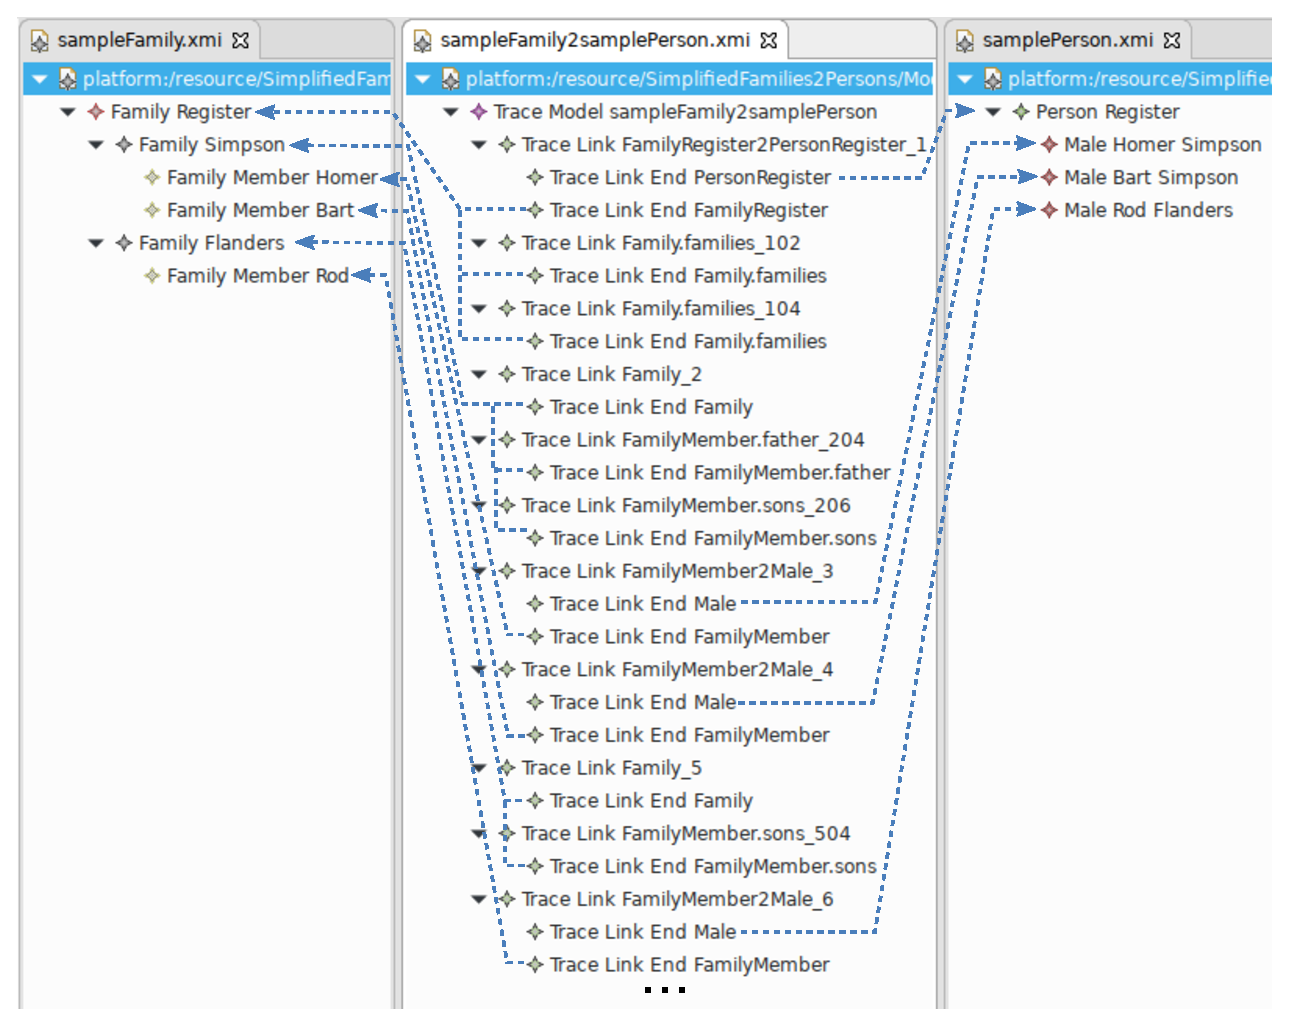
\includegraphics[width=.5\textwidth]{diagrams/solutions/jtl_fw}
	\caption{The forward execution of the Families to Persons case}
	\label{fig:jtl_fw}
\end{figure}


Note that, by re-applying the transformation in the backward direction it is possible to obtain again the original source model. The missing information about the original families and role of the members are restored by means of trace information.


After a refinement step, the target model including the changes described in Sect.~\ref{sec:example} is shown in the left part of Fig.~\ref{fig:3_bw2}. 
The modified model (shown in the left part of Fig.~\ref{fig:jtl_bw}) and the trace model obtained in the previous execution are given as input of the backward transformation execution.
Due to the non-determinism, more than one alternative models are generated. All the alternative models correctly restore families and roles of the members as in the original
source model, whereas, a new female (or male) is propagated both as a mother or a daughter (or a father or a son) in the existing family as well as in a new one. 
%
In the middle and right side of the figure, the generated models and a fragment of their traces are illustrated. 


\begin{figure}[h]
	\center
	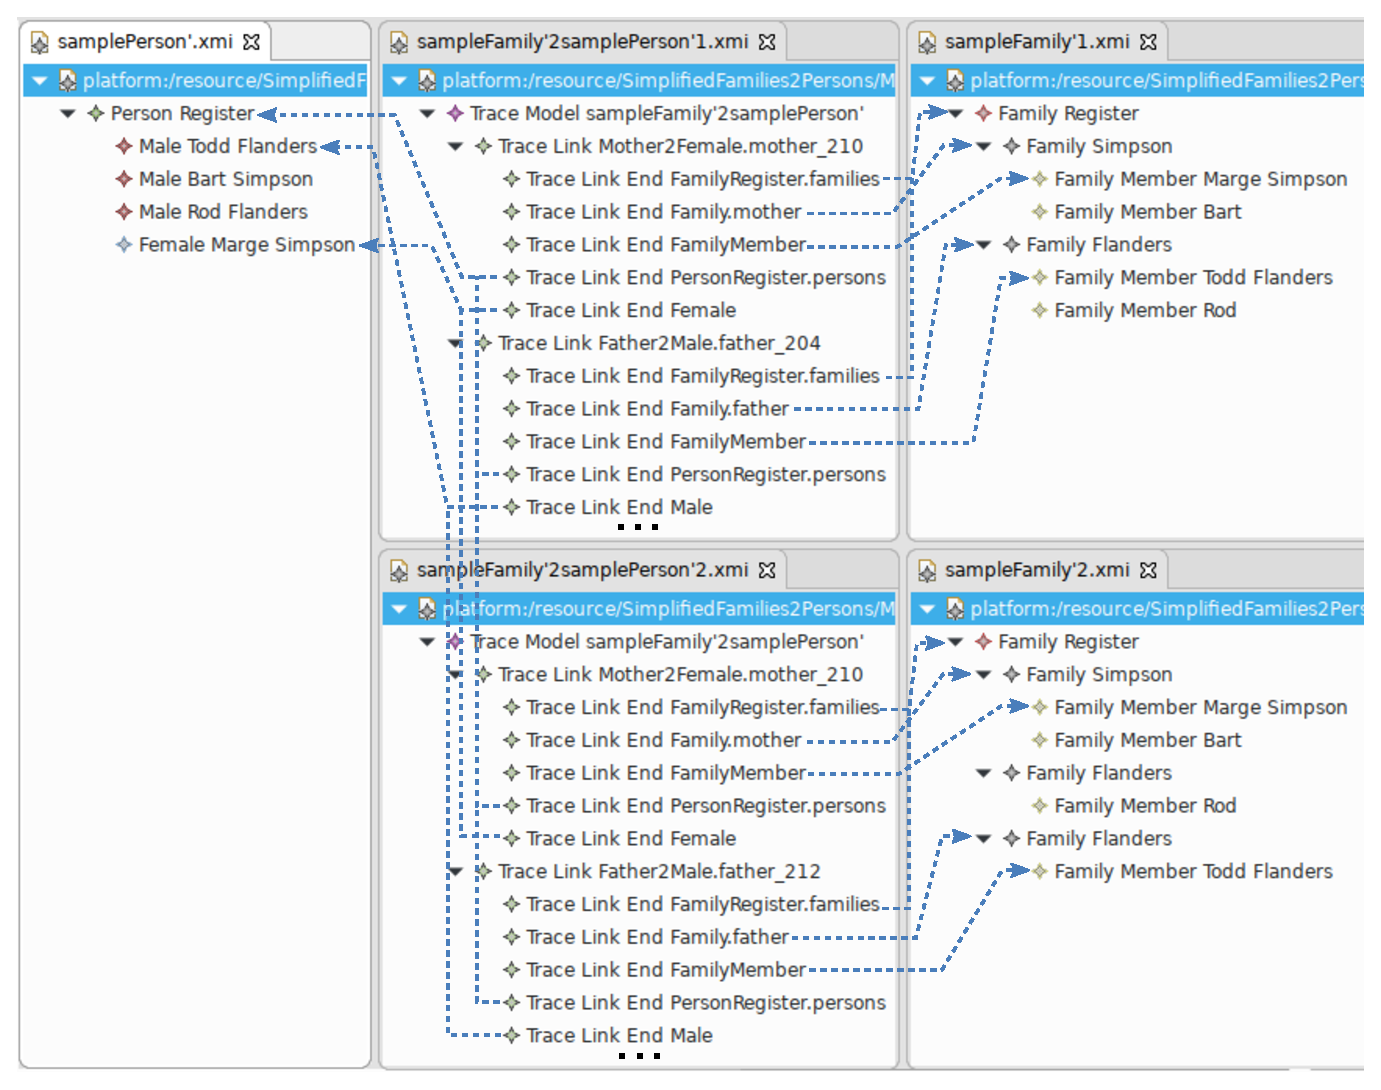
\includegraphics[width=.5\textwidth]{diagrams/solutions/jtl_bw}
	\caption{The backward execution of the Families to Persons case}
	\label{fig:jtl_bw}
\end{figure}


Note that, by selecting one of the alternative models and re-applying the transformation in the forward direction it is possible to obtain again the modified model. The missing information about the birthday attributes are restored by means of trace information, that is giving as input the trace model obtained in the previous forward execution. 